\documentclass{article}
\usepackage{amsmath}
\usepackage{amsthm}
\usepackage{amsfonts}
\usepackage{amssymb}
\usepackage[margin=0.5in]{geometry}
\usepackage[spanish, mexico]{babel}
\usepackage[utf8]{inputenc}
\usepackage{graphicx}

\begin{document}
	\title{Taller 5}
	\author{Miguel A. Gomez B.}
	\maketitle
\paragraph{1} Considere que se tienen dos bolsas. En la bolsa uno, hay cinco fichas marcadas con los números $0$, $1$, $2$, $3$ y $4$. en la bolsa dos hay seis fichas marcadas con los números  $0$, $2$, $4$, $6$, $8$ y $10$. Si se selecciona al azar y simultáneamente una ficha de cada bolsa hallar:

\subparagraph{a} Espacio muestral.

\paragraph{Respuesta}

\begin{align*}
	S = \{ &(0,0), (0,2), (0,4), (0,6), (0,8), (0,10), \\
	       &(1,0), (1,2), (1,4), (1,6), (1,8), (1,10), \\
   	       &(2,0), (2,2), (2,4), (2,6), (2,8), (2,10), \\
   	       &(3,0), (3,2), (3,4), (3,6), (3,8), (3,10), \\
   	       &(4,0), (4,2), (4,4), (4,6), (4,8), (4,10)
	    \}
\end{align*}

\subparagraph{b} Hallar la probabilidad de que la suma de los números sea a lo más de $6$.
\paragraph{Respuesta} Se realiza el conteo de las parejas que al ser sumadas son menores o iguales a 6, en base al espacio muestral estas son:

\begin{align*}
S_{x+y \leq 6} = \{ 
		&(0,0), (0,2), (0,4), (0,6),\\
		&(1,0), (1,2), (1,4),\\
		&(2,0), (2,2), (2,4),\\
		&(3,0), (3,2),\\
		&(4,0), (4,2)
\}
\end{align*}

Un total de $14$ elementos, por ende, la probabilidad esta dada por:

$$P((x+y)\leq6) = \frac{14}{30} = \frac{7}{15}$$

\subparagraph{c} Hallar la probabilidad de que el producto de los números sea menor a $5$.
\paragraph{Respuesta} Se realia el conteo de las parejas que al ser multiplicadas son menores a $5$, en base al espacio muestral estas son:

\begin{align*}
	S_{xy < 5} = \{
		&(0,0), (0,2), (0,4), (0,6), (0,8), (0,10), \\
		&(1,0), (1,2), (1,4),\\
		&(2,0), (2,2),\\
		&(3,0),\\
		&(4,0)
	\}
\end{align*}

Un total de $13$ elementos, por ende, la probabilidad esta dada por:

$$P((xy)<5) = \frac{13}{30}$$

\subparagraph{d} Dados los eventos:
\begin{itemize}
	\item{A}: Suma de los números menor o igual a cuatro.\\
		$$A = \{(0,0), (0,2), (0,4), (1,0), (1,2), (2,0), (2,2), (3,0), (4,0)\}$$
	\item{B}: Producto de los números igual a cero.\\
		$$B = \{(0,0), (0,2), (0,4), (0,6), (0,8), (0,10), (1,0), (2,0), (3,0), (4,0)\}$$
	\item{C}: Producto de los números mayor que ocho.\\
		$$C = \{(1,10),(2,6), (2,8), (2,10), (3,4), (3,6), (3,8), (3,10), (4,4), (4,6), (4,8), (4,10)\}$$
	\item{D}: Suma de los números es un número primo.\\
		$$D = \{(0,2), (1,2), (1,4), (1,6), (1,10), (2,0), (3,0), (3,2), (3,4), (3,8), (3,10)\}$$
\end{itemize}

Hallar:

\subparagraph{}$P(A \cup B)$

\paragraph{Respuesta}
$$A \cup B = \{(0,0), (0,2), (0,4), (0,6), (0,8), (0,10), (1,0), (1,2), (2,0), (2,2), (3,0), (4,0) \}$$
Un total de $12$ elementos, por lo tanto la probabilidad esta dada por:

$$P(A \cup B) = \frac{12}{30} = \frac{2}{5}$$

\subparagraph{}$P(A \cup D)$

\paragraph{Respuesta}
$$A \cup D = \{ (0,0), (0,2), (0,4), (1,0), (1,2), (1,4), (1,6), (1,10), (2,0), (2,2), (3,0), (3,2), (3,4), (3,8), (3,10), (4,0) \}$$

Un total de $16$ elementos, por lo tanto la probabilidad esta dada por:

$$P(A \cup D) = \frac{16}{30} = \frac{8}{15}$$

\subparagraph{}$P(\overline{C \cap D})$

\paragraph{Respuesta}

$$C \cup D = \{ (1,10), (3,4), (3,8), (3,10) \}$$

$$\overline{C \cap D} = S - (C \cup D)$$

\begin{align*}
\overline{C \cap D} = \{
	&(0,1), (0,2), (0,4), (0,6), (0,8), (0,10),\\
	&(1,0), (1,2), (1,4), (1,6), (1,8),\\
	&(2,0), (2,2), (2,4), (2,6), (2,8), (2,10),\\
	&(3,0), (3,2),        (3,6),\\
	&(4,0), (4,2), (4,4), (4,6), (4,8), (4,10)
\}
\end{align*}

Un total de $26$ elementos, por lo tanto la probabilidad esta dada por:

$$P(\overline{C \cap D}) = \frac{26}{30} = \frac{13}{15}$$

\newpage

\paragraph{2} Describa el espacio muestral resultante del lanzamiento de un dado y dos monedas.

\paragraph{Respuesta}

\begin{center}
	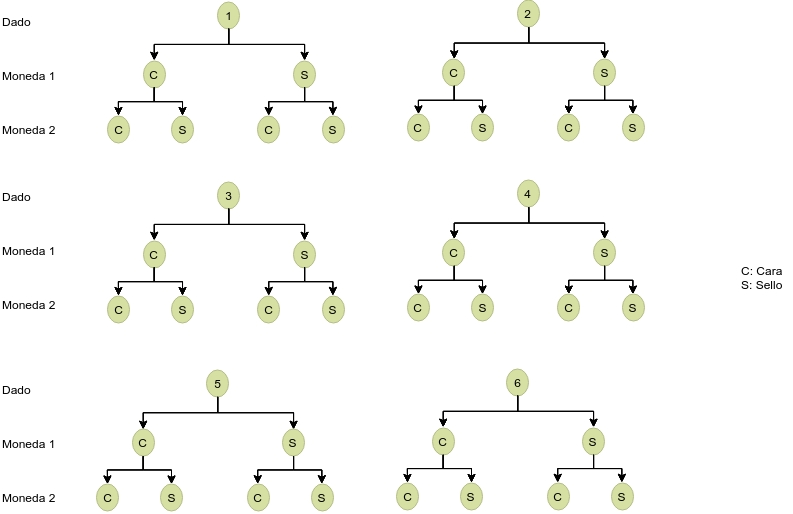
\includegraphics[width=0.9\textwidth]{1}
\end{center}

\paragraph{}el espacio muestral que representa este fenómeno es:

\begin{align*}
	S = \{ 
		&(1,C,C), (1,C,S), (1,S,C), (1,S,S),\\
		&(2,C,C), (2,C,S), (1,S,C), (1,S,S),\\
		&(3,C,C), (3,C,S), (3,S,C), (3,S,S),\\
		&(4,C,C), (4,C,S), (4,S,C), (4,S,S),\\
		&(5,C,C), (5,C,S), (5,S,C), (5,S,S),\\
		&(6,C,C), (6,C,S), (6,S,C), (6,S,S)
	\}
\end{align*}

\newpage

\paragraph{3} Se lanzan tres monedas simultáneamente, Hallar la probabilidad de:

\subparagraph{a} Obtener por lo menos dos caras.
\subparagraph{b} Obtener entre 1 y dos sellos.

\paragraph{Respuesta} Primero definimos el espacio muestral:

\begin{center}
	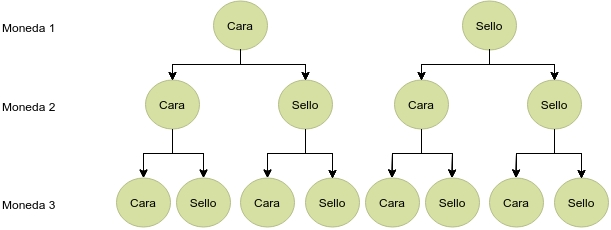
\includegraphics[width=0.9\textwidth]{2}
\end{center}

\paragraph{}el espacio muestral que representa este fenómeno es:

\begin{align*}
S = \{ 
	&(C,C,C), (C,C,S), (C,S,C), (C,S,S),\\
	&(S,C,C), (S,C,S), (S,S,C), (S,S,S)
\}
\end{align*}

donde C, es cara y S sello.

\paragraph{Respuesta(a)} La probabilidad de que se obtengan por lo menos dos caras se obtiene mediante un conteo sobre el espacio muestral:

$$S_{2c} = \{(C,C,C), (C,C,S), (C,S,C), (S,C,C) \}$$

Un total de $4$ elementos, por lo tanto la probabilidad de este evento esta dada por:

$$P(S_{2c}) = \frac{4}{8} = \frac{1}{4}$$

\paragraph{Respuesta (b)} La probabilidad de obtener entre 1 y dos sellos se obtiene mediante un conteo sobre el espacio muestral:

$$S_{S\leq2} = \{ (C,C,S), (C,S,C), (C,S,S), (S,C,C), (S,C,S), (S,S,C) \}$$

Un total de $6$ elementos, por lo tanto la probabilidad de este evento esta dada por:
$$P(S_{S\leq2}) = \frac{6}{8} =\frac{3}{4}$$

\newpage

\paragraph{4} en una bolsa se encuentran $20$ bolas azules, $10$ rojas y $8$ amarillas. Si se extrae una bola al azar, cuál es la probabilidad de:

\subparagraph{a} Que sea azul.

\paragraph{Respuesta} El conjunto de bolas, esta conformado por un total de $38$ bolas, de las cuales sabemos al menos $20$ son azules, luego, la probabilidad de que se obtenga una bola azul está dada por:

$$P(\text{bola azul}) = \frac{20}{38} = \frac{10}{19}$$

\subparagraph{b} Que sea azul o amarilla.

\paragraph{Respuesta} sumando la cantidad de bolas azules y amarillas obtenemos un total de $28$ bolas, por lo tanto la probabilidad de que se obtenga una amarilla o una azul esta dada por:

$$P(\text{bola amarilla o azul}) = \frac{28}{38} = \frac{14}{19}$$

\subparagraph{c} Que sea amarilla y gris.

\paragraph{Respuesta} No hay bolas que sean amarillas y grises por lo tanto:

$$P(\text{amarilla y gris}) = \frac{0}{38} = 0$$

\subparagraph{d} Que no sea verde.

\paragraph{Respuesta} Todas las bolas que existen en la bolsa no son de color verde, por lo tanto:

$$P(\text{bola no verde}) = \frac{38}{38} = 1$$

	
\end{document}